\section{Decision Tree Classifiers}
\begin{itemize}
	\item Idea of a Tree: 
	\begin{itemize}
		\item easy to read \& interpret
		\item robust, though lack of solid theoretical/statistical foundations
		\item can use with Ensemble-Methods
	\end{itemize}
\end{itemize}

\subsection{Setup of a Decision Tree}
\begin{itemize}
	\item internal node: test on a \textbf{attribute}
	\item branch: outcome of the test (eg: true/false, red/green)
	\item leaf node: the \textbf{classification label/result}
\end{itemize}

Building an \textbf{Optimal} Decision Tree:
\begin{itemize}
	\item Search Space: $2^{2^m}$ possible trees (m: \# attributes, 2 result classes)
	\item Complexity: \textbf{NP-complete}
	\item Solution: \textbf{Greedy Algorithm} in \textbf{top-down} approach
	\begin{itemize}
		\item All training data at the \textbf{root}.
		\item Partition data \textbf{recursively} by choosing \textbf{one attribute} at each level.
		\item Each split is assessed with a \textbf{measure}
		\item Attribute with \textbf{best split} is chosen.
		\item Repeat until all \textbf{leaf nodes} are pure (Not all attributes are necessary).
	\end{itemize}
\end{itemize}

\subsection{Quality Metrics of a Splitting Attribute}
\begin{itemize}
	\item Idea: 
	\begin{itemize}
		\item the path to classification \textbf{as easy as possible}. $\rightarrow$ \textbf{smallest} tree
		\item good separation of classes $\rightarrow$ leaf nodes gives \textbf{one single class} $\rightarrow$ direct decision
		\item the separation shouldn't affect class distribution.
	\end{itemize}
	\item Evaluation function:
	\begin{itemize}
		\item \textbf{information gain (ID3/C4.5)}
		\item \textbf{information gain ratio}
		\item \textbf{gini index (CART)}
	\end{itemize}
\end{itemize}

\subsubsection{Information Gain}
\begin{itemize}
	\item Idea: choose the attribute that result in \textbf{smallest tree} $\rightarrow$ \textbf{purest} nodes (one class)
	
	$\rightarrow$ choose the attribute with \textbf{greatest information gain}
	
	$\rightarrow$ information gain $\uparrow$, subset average purity $\uparrow$
	
	
	\item Parameters:
	\begin{itemize}
		\item $c_i$: the \textbf{absolute frequency} of the training examples in the class $i$
		\item $C$: the \textbf{total number} of training example at the \textbf{current stage/attribute value}.
		\item $p_i$: the \textbf{relative frequency} of class $i$, $$p_i = \frac{c_i}{C}$$
		\item $N$: the \textbf{total number of training data}
	\end{itemize}
\end{itemize}

\paragraph{Process: }
\begin{enumerate} [label= \protect \circled{\arabic*} ]
	\item calculate \textbf{initial information} before any splits.
	\item calculate \textbf{information for each attribute value} using entropy
	\paragraph{Entropy} $\in [0,1]$, measures how much \textbf{additional information required} in \textbf{bits}
	$$\text{entropy}(p_1, \dots, p_n) = - \Sigma_{i=1} ^n p_i \cdot \log_{2} p_i$$
	\begin{itemize}
		\item entropy = 0: pure
		\item entropy = 1: maximum impurity (for boolean)
	\end{itemize}
	\paragraph{Information of Each Attribute Value} 
	
	$$\text{info}([c_1, \dots, c_n]) = \text{entropy}(\frac{c_1}{C}, \dots, \frac{c_n}{C})$$ 
	\item calculate \textbf{information of the attribute} 
	\paragraph{Information of the Attribute} the \textbf{weighted average} of the \textbf{information needed} from each attribute value. 
	
	Say an attribute has $m$ attribute values/branches,
	
	$$\text{info}([c_1, \dots, c_n]_1, \dots, [c_1, \dots, c_n]_m) = \Sigma_{i=1}^m  \frac{C_m}{N} \cdot \text{info}([c_1, \dots, c_n])_m$$
	
	
	\item calculate the \textbf{information gain}	
	
	\paragraph{Information Gain of the Attribute} 
	
	$$\text{Information\_Gain(attribute)} = \text{info(before split by attribute)} - \text{info(after split by attribute)}$$ 
	
	\item choose the attribute with \textbf{maximum} information gain. 
	\item continue to split. 
	
	\textbf{Attention}: the info \textbf{before} the split is the \textbf{info(attribute value)}, the information gain of the attribute changes to 
	
	eg: gain(Temperature) = \textbf{info(Outlook = sunny)} - info(high, mild, cool)
\end{enumerate}

\paragraph{Limitations}
\begin{itemize}
	\item \textbf{biased} against \textbf{highly-branching} attributes (eg: IDs)
	
	$\rightarrow$ overfitting
	
	$\rightarrow$ Alternative: \textbf{Gain Ratio}
\end{itemize}

\subsubsection{Gain Ratio}
\begin{itemize}
	\item Idea: modification of information gain, reduce bias on highly-branching attributes.
	
	$\rightarrow$ considers \textbf{number and size} of branches $\rightarrow$ \textbf{intrinsic information} of attribute
	
	\item \textbf{Intrinsic Information}, s: size of a leaf from each branch
	$$\text{intrinsic\_info}([s_1, \dots, s_n]) = \text{info}([s_1, \dots, s_n])$$
	eg: 14 IDs, intrinsic\_info([1,1,...,1]) = info([1,1,...,1]) = $14 \cdot (-\frac{1}{14} \cdot \log_{2} \frac{1}{14}) = 3.807$ bits 
	
	\item \textbf{Gain Ratio}: 
	
	$$\text{Gain\_Ratio(attribute)} = \dfrac{\text{Gain(attribute)}}{\text{Intrinsic\_Info(attribute)}}$$
	
	\item Process:
	\begin{itemize}
		\item calculate the \textbf{information gain} of the attribute
		\item calculate the \textbf{intrinsic information} of the attribute
		\item calculate the \textbf{gain ratio}
		\item choose the attribute that has \textbf{maximium} the gain ratio.
	\end{itemize}
\end{itemize}

\subsubsection{Gini Index}
\begin{itemize}
	\item Use-case: in Classification and Regression Tree (CART)
	\item Solution: select the split that \textbf{decreases} the Gini Index \textbf{the most}.
	\item \textbf{Gini Index}: 
	$$Gini(S) = 1 - P^2 - N^2$$
	$$P = \frac{p}{p+n}, N = \frac{n}{p+n}$$
	\item a dataset S is split into $S_1, S_2$, 
	$$Gini_{split} (S_1,S_2) = \frac{p_1 + n_1}{p+n} \cdot Gini(S_1) + \frac{p_2 + n_2}{p+n} \cdot Gini(S_2)$$
	
	$\rightarrow$ select the attribute with \textbf{lowest} Gini-Index after split.
\end{itemize}

\subsection{Evaluation of Decision Tree Algorithm}
\begin{itemize}
	\item Time Complexity: $\mathcal{O}(m\cdot n \log n)$
	
	(m: \# attributes, n: \# instances)
	\item Scalability for large data:
	\begin{itemize}
		\item number of attributes $\uparrow$, tree size $\uparrow$, computation time $\uparrow$.
		\item number of data instances $\uparrow$, memory $\uparrow$
	\end{itemize} 
\end{itemize}

\subsection{Possible Problems in Prediction}
\subsubsection{Numeric Attributes in Dataset}
\begin{itemize}
	\item Solution: \textbf{binary split}
	\item Process:
	\begin{itemize}
		\item an \textbf{initial split point} is either given or the middle of the sorted numeric values.
		\item values are separated into 2 sections: \textbf{below(<)} and \textbf{above($\geq$)} the split point.
		\item calculate \textbf{information gain}
		\item repeat \textbf{binary split}, choose the split with \textbf{maiximum information gain}. 
	\end{itemize}
\end{itemize}

\subsubsection{Missing Values in Dataset}
\begin{itemize}
	\item Possible solutions:
	\begin{itemize}
		\item \textbf{ignore} the instance/attribute with missing values.
		\item treat missing value as \textbf{another nominal value}.
		\item \textbf{estimate} missing values (regression, imputation)
		\item \textbf{follow the leader}: if an instance has missing attribute value, follow the the \textbf{branch with most instances}.
		\item \textbf{partition} the instance: send down instance \textbf{proportionally} to the number of instances. 
		
		$\rightarrow$ classification result is \textbf{weighted}.
	\end{itemize}
\end{itemize}

\subsubsection{Overfitting of the Decision Tree}
\begin{itemize}
	\item Consequences in Overfitting:
	\begin{itemize}
		\item decision tree to \textbf{large \& complex}
		\item \textbf{low bias} on training set, \textbf{high variance} on test set.
		\item poor generalization to new data.
	\end{itemize}
	\item Solution: Pruning 
\end{itemize}

\subsection{Pruning of Decision Trees}
\subsubsection{Prepruning}
Process:
\begin{itemize}
	\item define a \textbf{threshold} when to stop creating subtrees. This should be the same measure as determining attributes (eg: information gain)
	\item \textbf{stop} if the measure \textbf{no longer exceeds threshold}. (eg: infomation gain)
	\item leaf node: the \textbf{most frequent class}
\end{itemize}
Difficult to achieve high performance in practice.

\subsubsection{Postpruning}
\begin{itemize}
	
	\item Process: 
	\begin{itemize}
		\item construct a \textbf{complete} decision tree.
		\item prune back by \textbf{subtree replacement}, replacing the subtree with \textbf{a single leaf node}.
		\item prune back criteria: \textbf{error rate} estimate for the \textbf{node} < \textbf{combined error rates} of the \textbf{children(weighted average)} 
		
		\begin{figure}[H]
			\centering
			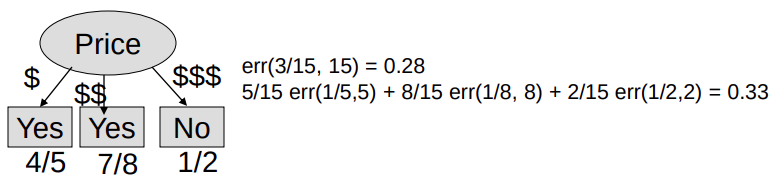
\includegraphics[width=0.65\textwidth]{prune.png}
		\end{figure}
		$\rightarrow$ error rate of the node = 0.28 < combined error rate of the children = 0.33 
		
		$\rightarrow$ prune back, the leaf node is the \textbf{most frequent class}.
	\end{itemize}
	\item Use-case: C4.5, CART, however, computationally expensive
	\item Data for pruning:
	\begin{itemize}
		\item hold-out set: an \textbf{independent} dataset from the training data. Best, but not practical when data is scarce.
		\item training data: Used in C4.5, derive \textbf{outer bound of confidence interval} from data, use a \textbf{heuristic limit} for error rate. If the \textbf{error rate is outside the confidence interval} $\rightarrow$ \textbf{prune} back. 
		
		$\rightarrow$ confidence limit c $\downarrow$ (25\% -> 10\%), the tree prunes \textbf{stronger}.
	\end{itemize}
\end{itemize}



